\textbf{\underline{OZ 9 - Wisselstroomkringen - Oefening 5:}}
\vspace{0.5cm}

\vspace{-0.5cm}\begin{minipage}{.66\textwidth}
    In onderstaande circuit, bepaal de rms stroom door de $45.0 \ \text{V}$ (rms) bron wanneer
    \begin{enumerate}[(a)]
        \item de frequentie heel groot is,
        \item de frequentie heel klein is.
    \end{enumerate}
\end{minipage}
\begin{minipage}{.3\textwidth}
    \hspace{0.5cm}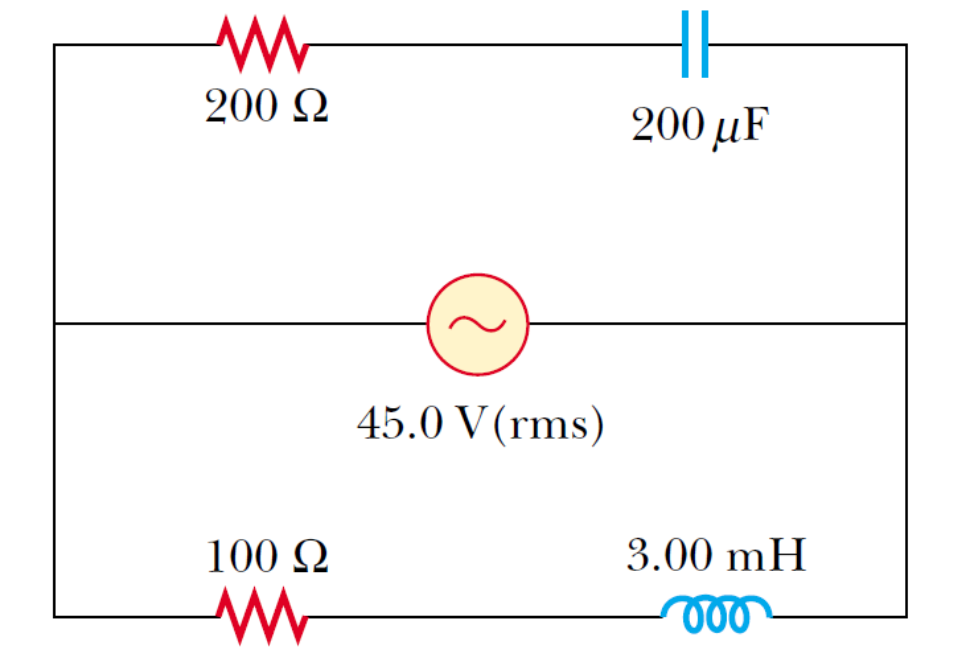
\includegraphics[scale = 0.3]{oz09/resources/Oz9Oef5.png}
\end{minipage}

\begin{enumerate}[(a)]
    \item
        \begin{description}[labelwidth=1.5cm, leftmargin=!]
            \item[Geg. :] $\omega$ is heel groot
            \item[Gevr. :] $I$ ?
            \item[Opl. :]  
                Bij heel grote frequentie gaat de inductor geen stroom toelaten en zal dus alle stroom langs boven gaan. We kunnen de stroom berekenen die door de bovenste weerstand gaat:
                \begin{equation*}
                    I = \frac{45}{200} = 225 \ \text{mA}.
                \end{equation*}
        \end{description}
    \item 
        \begin{description}[labelwidth=1.5cm, leftmargin=!]
            \item[Geg. :] $\omega$ is heel groot
            \item[Gevr. :] $I$ ?
            \item[Opl. :]   
                Bij heel lage frequentie gaat de condensator geen stroom toelaten en zal dus alle stroom langs onder gaan. We kunnen dus de stroom berekenen die door de onderste weerstand gaat:
                \begin{equation*}
                    I = \frac{45}{100} = 450 \ \text{mA}.
                \end{equation*}
        \end{description}
\end{enumerate}

\vspace{1cm}